\chapter{基于分布的频率分析攻击方法}
\label{sec:DistributionAttack}

基于分布的攻击利用$\mathbf{C}$和$\mathbf{A}$的数据块的逻辑顺序信息来增强频率分析的有效性。它通过比较$\mathbf{C}$和$\mathbf{A}$的相对频率分布,以减少误报结果。本文还展示了如何利用数据块的大小信息来进一步提高推断精度。

\section{背景知识:基于数据块局部性的频率分析的攻击}

\label{sec:DistributionAttack-prior-attack}

基于分布的频率分析攻击建立在已有的基于数据块局部性的频率分析攻击\cite{li2017information}的基础上,它展示了频率分析如何导致备份工作负载中的信息发生泄漏。基于数据块局部性的频率分析攻击针对每日或每周为主要数据的完整副本(例如,应用程序状态,文件系统快照和VM磁盘映像)创建的完全备份(简称为备份)。它旨在推断不同版本备份间的密文数据块-明文数据块对。它通过假定辅助信息$\mathbf{A}$来自一些较旧的备份,来推断最新备份的明文数据块(即$\mathbf{M}$)。

基于数据块局部性的频率分析攻击利用了数据块局部性这一属性\cite{xia2011silo,zhu2008avoiding,lillibridge2009sparse},这是实际备份工作负载中的常见现象。 具体而言,局部性是指在重复数据删除之前,相邻的数据块在不同版本的备份中往往以相同的逻辑顺序存在。 主要原因是每个备份的更新通常聚集在一些小范围内的数据块中,而剩余的大范围内的数据块在不同版本的备份中保持不变(保持相同的顺序)。

根据局部性原理,基于数据块局部性的频率分析攻击利用逻辑顺序信息来发现密文数据块和明文数据块的邻近信息。具体来说,对于给定的唯一密文数据块$C$,对手首先标识所有相同副本的集合$\{\hat{C}^{(i)}\}$。对于每个$\hat{C}^{(i)}$,它会考虑$\hat{C}^{(i)}$的左右邻居,即$\hat{C}^{(i-1)}$和$\hat{C}^{(i+1)}$。它将左右邻居的集合分别提取到关联数组$\mathbf{L_C}$和$\mathbf{R_C}$中。关联数组分别存储每个唯一密文$C$的映射及其与左右邻居的共现频率。同时,对手还会根据$\mathbf{A}$的逻辑顺序信息构造关联数组$\mathbf{L_A}$和$\mathbf{R_A}$。

然后,基于数据块局部性的频率分析攻击通过每个推断的密文数据块-明文数据块对的邻居进行迭代频率分析。它首先在$\mathbf{C}$(将要进行推测的密文数据块集合)和$\mathbf{A}$(辅助信息-明文数据块的集合)中通过频率分析推断得到出现频率最高的$u$组密文数据块-明文数据块对\{$(C,M)$\}($u$是该攻击开始时用于选取明密文数据块对数量的参数,一般设为5)。因为基于观察得到高频率数据块的频率等级(相对排名)在不同版本的备份中是稳定的,所以推断结果可能是真实的(即,目标密文数据块与推断的明文数据块是正确的唯一映射)。对于每个推断的明密文数据块对$(C,M)$,攻击发现它们的左右邻居$C$和$M$的共现频率最高,由于局部性的原因,$M$的左右邻居可能分别是$C$的相应左右邻居的原始明文数据块。因此,将$C$和$M$的最高频率左(右)邻居添加到推断的密文数据块-明文数据块对的集合中(从存储密文数据块$C$的左右邻居的集合的关联数组$\mathbf{L_C}$和$\mathbf{R_C}$中获得;对于辅助信息:明文数据块$A$,同理,从$\mathbf{L_A}$和$\mathbf{R_A}$中获得)。最后,不断迭代此过程,直到检查完每个推断得到的的密文数据块-明文数据块对的邻居。

因为数据块的顺序由数据块局部性保留,所以它可以使用频率分析来推断在相应的邻居中具有相同的共现频率等级的新的密文数据块-明文数据块对。$M$的左右邻居可能是$C$的相应邻居的原始明文。因此,攻击通过这些新推断的密文数据块-明文数据块对的邻居进一步迭代相同的频率分析,从而增加攻击的严重性。


%\begin{algorithm}
%\caption{Locality-based Attack}
%\label{alg:Locality-basedAttack}
%\small
%   \SetKwFunction{Main}{\sc LOCALITY-BASED ATTACK}
%   \SetKwProg{Pro}{procedure}{:}{}
% 	\Pro{\Main{$C,M,u,v,w$}}{
% 	
% 	$(F_C, L_C, R_C) \longleftarrow COUNT(C)$\;
% 	$(F_M, L_M, R_M) \longleftarrow COUNT(M)$\;
%
%	\If{ciphertext-only mode}{
% 		$\\mathcal{G} \longleftarrow FREQ-ANALYSIS(F_C, F_M, u)$\;
% 	}
% 	\ElseIf{known-plaintext mode}{
% 		$\mathcal{G} \longleftarrow set of leaked ciphertext-plaintext chunk pairs$\;
% 	}
% 	$\mathcal{T} \longleftarrow \mathcal{G}$\;
% 	\While{$\mathcal{G}$ is non-empty}{
%        Remove $(C,M)$ from $\mathcal{G}$\;
% 	  
%        $\mathcal{T}_l \longleftarrow FREQ-ANALYSIS(L_C[C],L_M[M],v)$\; 
%    }
%
%
%\end{algorithm}

然而,基于数据块局部性的频率分析攻击存在一个主要问题:它引入了大量误报(即,不正确的密文数据块-明文数据块对)。 由于频率分析的主要思想是将密文映射到具有相同频率等级的明文,因此对频率等级的任何干扰(例如,跨备份的更新)都可能导致推断出不正确的密文数据块-明文数据块对,这又将导致对其邻居的推断发生错误。虽然基于数据块局部性的频率分析攻击被证明可以有效地推断出真正的密文数据块-明文数据块对的很大一部分,但是对手对于判断每个推断的密文数据块-明文数据块对的真实性置信度较低。例如,根据评估显示,攻击可以在某些情况下可以正确地推断出15.2%的密文数据块-明文数据块对,但在其推断结果中大约65.2%的推断结果是错误的。 


基于数据块局部性的频率分析攻击方法对频率排名非常敏感,如果频率排序受到任何干扰都会极大的降低推断精度。而这些推断错误的明密文数据块对将会干扰到对其相邻数据块的推断迭代过程,导致错误更加严重。即使通过下调参数$u$的大小来限制返回数据块的数量,以提高推断的正确率(仅将频率显著高于其他数据块对的数据块对返回),但会导致推利率的严重下滑(推断得到的数据块对总数大幅减少)。

\section{基于分布的频率分析攻击方法定义}
\label{sec:distribution-attack-description}

基于分布的频率分析攻击的攻击扩展了基于数据块局部性的频率分析攻击\cite{li2017information}以显著消除误报。它利用备份工作负载中的数据块局部性性,就像基于数据块局部性的攻击一样。在基于数据块局部性的攻击的基础上,对于$\mathbf{C}$中的每个唯一密文$C$,根据该数据块与其邻居的共现频率来测量其相对频率分布;同时,用同样的方法计算$\mathbf{A}$中每个唯一明文$M$的相对频率分布。根据观察,对于推断正确的密文数据块-明文数据块对$(C,M)$,$C$和$M$应该具有相似的相对频率分布(即,它们与它们各自的邻居的共现频率是相似的)。对于此的理解是,如果$M$是$C$的原始明文,那么$M$和$C$的相对频率分布可能是相似的。 基本原理是$\mathbf{A}$和$\mathbf{C}$从同一个源映射得到,因此具有大量未被修改的数据块,所以相对频率分布得到保留。本文将此观察视为局部性属性的更一般化概念,并根据该条件过滤可能不正确的密文数据块-明文数据块对,以提高推断的准确性。

\begin{figure}[!htb]
    \small
    \centering
    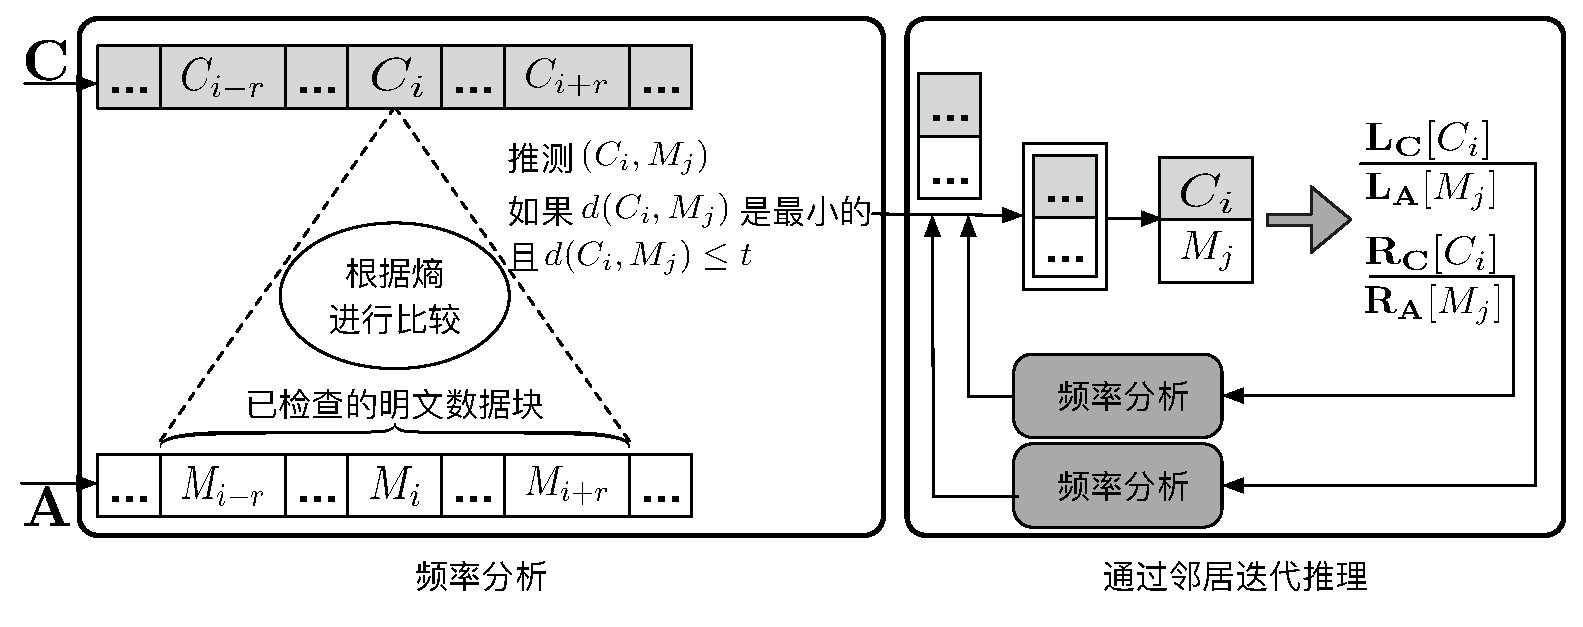
\includegraphics[width=14cm]{DistributionAttack}
    \caption{基于分布的频率分析攻击工作流程} 
    \label{fig:基于分布的频率分析攻击工作流程}
\end{figure}

图\ref{fig:基于分布的频率分析攻击工作流程}展示了基于分布的频率分析攻击方案的工作流程。

首先按$\mathbf{C}$和$\mathbf{A}$中的频率对具有唯一性的密文和明文进行排序。 与基于数据块局部性的频率分析攻击\cite{li2017information}一样,通过参数$u$将基础频率分析配置为最多返回$u$个频率最高的明密文数据块对。

接下来,对于每个具有唯一性的密文数据块$C_i$(其中$i, 1 \leq i \leq u$,代表了该密文数据块的频率排名),检查相近频率排名范围内明文数据块$M_{i-r}, \ldots, M_i, \ldots, M_{i+r}$(从$i-r$到$i+r$),其中$r$是可配置参数(默认为10),表示可以解决的频率排名干扰的最大范围。

对于每个$C_i$(其中$1 \leq i \leq u$)和相应的$M_j$(其中$i-r\le j\le i+r$),我们通过熵来表示它们的相对频率分布,熵是信息理论中的一个关键概念,用于衡量随机来源产生的信息量。在这里,我们采用熵来量化概率分布的随机性\cite{wang08}。 具体来说,我们定义了两个随机变量,分别用$X$和$Y$来描述$C_i$与其左右邻居的共现事件,这样事件“$X = C$” 表示$C$是$C_i$的左邻居,而事件$Y = C$表示$C$是$C_i$的右邻居。 因此,我们基于$\mathbf{L_C}$和$\mathbf{R_C}$来计算两个事件发生的概率:

\begin{eqnarray}
    \Pr[X = C] = \frac{\mathbf{L_C}[C_i][C]}{\sum_{C' \in \mathbf{L_C}[C_i]} \mathbf{L_C}[C_i][C']}, \nonumber \\
    \Pr[Y = C] = \frac{\mathbf{R_C}[C_i][C]}{\sum_{C' \in \mathbf{R_C}[C_i]} \mathbf{R_C}[C_i][C']}, \nonumber
\end{eqnarray}

其中$\mathbf{L_C}[C_i]$和$\mathbf{R_C}[C_i]$分别了存储$C_i$的左右邻居,而$\mathbf{L_C}[C_i][C']$和$\mathbf{R_C}[C_i][C']$存储$C_i$与其左右邻居$C'$的共现频率。$X$和$Y$都遵循$C_i$的相对频率分布,本文用$e(\mathbf{L_C}[C_i])$和$e(\mathbf{R_C}[C_i])$表征它们的随机性,分别为:

\begin{eqnarray*}
    e(\mathbf{L_C}[C_i]) = \sum_{C \in \mathbf{L_C}[C_i]} \log_2\frac{1}{\Pr[X = C]}, \\
    e(\mathbf{R_C}[C_i]) = \sum_{C \in \mathbf{R_C}[C_i]} \log_2\frac{1}{\Pr[Y = C]}. 
\end{eqnarray*}

类似的,本文根据$\mathbf{L_A}$和$\mathbf{R_A}$对每个明文数据块$M_j$(其中$i-r\le j\le i+r$)计算出其对应的熵$e(\mathbf{L_A}[M_j])$和$e(\mathbf{R_A}[M_j])$,然后本文利用欧几里得距离来量化$C_i$和$M_j$的相对频率分布的相似性,记为$d(C_i, M_j)$:

\begin{equation}
    \label{eq:dis-dcm}
    \centering
    d(C_i, M_j) = \sqrt{[e(\mathbf{L_C}[C_i]) - e(\mathbf{L_A}[M_j])]^2 + [e(\mathbf{R_C}[C_i]) - e(\mathbf{R_A}[M_j])]^2}.
\end{equation}

显然,只有当他们的熵的欧几里德距离$d(C_i, M_j)$很小时,$C_i$和$M_j$才有相似的相对频率分布。因此,如果满足以下条件,则可将$(C_i, M_j)$标识为推断成功的密文数据块-明文数据块对:

\begin{itemize}
\item \textbf{R1:} $d(C_i, M_j)$ 在$j \in i-r \leq j \leq i+r$ 中取到最小值。
\item \textbf{R2:} $d(C_i, M_j)$ 不大于预先设定的变量$t$(例如,$t$的默认值为1)。
\end{itemize}

值得注意的是,$C_i$所对应的原始明文数据块可能不在检查的明文数据块$M_{i-r}, \ldots, M_{i+r}$的范围内。在这种情况下,部分$M_j$($i-r \leq j \leq i+r$)可能仍然满足条件R1。这种情况下,本文希望通过R2过滤不正确的密文数据块-明文数据块对。 

然后,继续采用先前基于数据块局部性的频率分析攻击\cite{li2017information}中的迭代方法(参见章节:\ref{sec:DistributionAttack-prior-attack})来扩展推断的密文数据块-明文数据块对的覆盖范围。具体来说,对于每个推断的$(C_i, M_j)$,应用基于分布的频率分析方案(见上文)通过$C_i$和$M_j$的邻居迭代推断出更多的密文数据块-明文数据块对,在没有新的密文数据块-明文数据块对可以被推断时停止迭代,最终完成基于分布的频率分析攻击的全部过程。

\subsection{本算法的细节描述}
 The distribution-based attack builds on prior locality-based attack \cite{li17} (see \S\ref{sec:locality}), and uses the robust frequency ranking approach to infer ciphertext-plaintext chunk pairs. We modify the parameters of the locality-based attack \cite{li17}. First, we remove the parameter (i.e., $w$ in \cite{li17}) of size of $\mathcal{G}$, as we find the memory can hold all fingerprints of our experimental datasets (see \S\ref{sec:methodology}). Second, we replace another parameter (i.e., $v$ in \cite{li17}) that bounds the number of chunk pairs returned by frequency analysis in each iteration, by $r$ to indicate the possible plaintext chunks to be examined.     

 Algorithm~\ref{alg:distribution} presents the pseudo-code of the distribution-based attack, where we assume the adversary can construct the associative arrays $\mathbf{F_C}, \mathbf{L_C}$, and $\mathbf{R_C}$, as well as $\mathbf{F_M}, \mathbf{L_M}$, and $\mathbf{R_M}$ by calling $\textsc{Count}(\mathbf{C})$ and $\textsc{Count}(\mathbf{C})$, respectively. We omit the algorithm details about $\textsc{Count}$, and readers may refer the function of the same name in ref. \cite{li17}. 

 The algorithm \textsc{Distribution-attack} takes $\mathbf{C}, \mathbf{M}, u$ and $r$ as input, and outputs $\mathcal{R}$ of inferred ciphertext-plaintext chunk pairs. After initializing the associative arrays of $\mathbf{F_C}, \mathbf{L_C}$ and $\mathbf{R_C}$, it calls the function \textsc{Entropy} to obtain $\mathbf{E_C}$ which maps each ciphertext chunk to its entropies derived from the relative frequency distributions of its left and right neighbors (Line~4). Similarly, it obtains $\mathbf{E_M}$ for the plaintext chunks (Line~6). Then, it calls the \textsc{Robust-ranking} function to initialize $\mathcal{G}$ and $\mathcal{R}$ (Line~7-8). 

 In each iteration, the algorithm picks out a pair $(C, M)$ from $\mathcal{G}$ (Line~10), and calls the function $\textsc{Robust-ranking}$ to infer ciphertext-plaintext chunk pairs $\mathcal{R}_r$ and $\mathcal{R}_l$ from the left and right neighbors of $C$ and $M$ (Line~11-12). It further adds the newly inferred pairs of $\mathcal{R}_l$ and $\mathcal{R}_r$ into $\mathcal{G}$ and $\mathcal{R}$ (Line~13-15). The iteration does not end until $\mathcal{G}$ is empty. The algorithm finally returns $\mathcal{R}$ (Line~16).    

The function \textsc{Entropy} builds the entropy array $\mathbf{E}_{\rm X}$ based on $\mathbf{L}_{\rm X}$ and $\mathbf{R}_{\rm X}$, where the X can be "tar" or "aux". For each chunk $X$, it counts the total co-occurrences $\Sigma_l$ of all left neighbors of $X$ (Line~20), and further the entropy $\mathbf{E}_{\rm X}[X].l$ of the relative frequency distribution of left neighbors (Line~21-22). Similarly, it counts the entropy $\mathbf{E}_{\rm X}[X].r$ of the relative frequency distribution of right neighbors (Line~23-25).     

The function \textsc{Rank} performs robust frequency ranking based on $\mathbf{X}_{\rm tar}$ and $\mathbf{X}_{\rm aux}$, where $\mathbf{X}_{\rm tar}$ and $\mathbf{X}_{\rm aux}$ can be $\mathbf{F}_{\rm tar}$ and $\mathbf{F}_{\rm aux}$, $\mathbf{L}_{\rm tar}[*]$ and $\mathbf{L}_{\rm aux}[*]$, or $\mathbf{R}_{\rm tar}[*]$ and $\mathbf{R}_{\rm aux}[*]$. It first sorts $\mathbf{X}_{\rm tar}$ and $\mathbf{X}_{\rm aux}$ by frequencies, respectively (Line~29-30). For each $i$-th frequent ciphertext chunk $C_i$, it identifies the range of plaintext chunks to be examined. Specifically, if the flag $f$ is INIT, it sets the starting rank $m$ as the maximum number of $1$ and $i-r$, since $i$ may be smaller than $r$ (Line~34-35); if $f$ is ITERA, it sets $m$ as $i$ (Line~36-37). Then, it finds the plaintext chunk $M$ in the examined range, such that ${\sf D}(C_i, M)$ is minimum (Line~38-42). The function adds $(C_i, M)$ into the result set $\mathcal{R}_x$ only when the distance ${\sf D}(C_i, M)$ is also smaller than the threshold $t$ (Line~43-44). 


Note that \textsc{Robust-ranking} also returns $u$ highly frequent chunk pairs like locality-based attack \cite{li17}. Similarly, it sorts  For each top-frequent ciphertext chunk $C$ with a rank of $i$ ($1 \leq i \leq u$), it examines the cor:responding plaintext chunks that rank range from $i-r$ to $i+r$. Since $i-r$ is possibly below the first rank index, the algorithm derives the minimum rank $start$ of $1$ and $i-r$ and          


\begin{algorithm}[H]
\caption{Distribution-based Attack}
\label{alg:distribution-attack}
\small
   \SetKwFunction{Main}{\sc Distribution-Attack}
   \SetKwProg{Pro}{procedure}{:}{}
 	\Pro{\Main{$u, r, t, \mathcal{L}_{\rm order}, \mathbf{M}_{\rm aux}$}}{
 		initialize $\mathcal{R} \longleftarrow \emptyset$\; 

 		extract $\mathbf{F}_{\rm tar}, \mathbf{L}_{\rm tar}$ and $\mathbf{R}_{\rm tar}$ from $\mathcal{L}_{\rm order}$\;
 		 \tcc{$\mathbf{F}_{\rm tar}[C]$ maps $C$ to frequency of its original chunk in $\mathbf{M}_{\rm tar}$}
 		 \tcc{$\mathbf{L}_{\rm tar}[C]$ maps ciphertext chunk $C$ to its left neighbors as well as corresponding co-occurrences with $C$}
 		 \tcc{$\mathbf{R}_{\rm tar}[C]$ maps ciphertext chunk $C$ to its right neighbors as well as corresponding co-occurrences with $C$}

 		extract $\mathbf{F}_{\rm aux}, \mathbf{L}_{\rm aux}$ and $\mathbf{R}_{\rm aux}$ from $\mathbf{M}_{\rm aux}$\;
 		 \tcc{$\mathbf{F}_{\rm aux}[M]$ stores frequency of plaintext chunk $M$ in $\mathbf{M}_{\rm aux}$}
 		 \tcc{$\mathbf{L}_{\rm aux}[M]$ maps plaintext chunk $M$ to its left neighbors and corresponding co-occurrences with $M$}
 		 \tcc{$\mathbf{R}_{\rm aux}[M]$ maps plaintext chunk $M$ to its right neighbors and corresponding co-occurrences with $M$}

 		$\mathbf{E}_{\rm tar} \longleftarrow \textsc{Entropy}(\mathbf{L}_{\rm tar}, \mathbf{R}_{\rm tar})$\;
 		$\mathbf{E}_{\rm aux} \longleftarrow \textsc{Entropy}(\mathbf{L}_{\rm aux}, \mathbf{R}_{\rm aux})$\;

 		$\mathcal{G} \longleftarrow \textsc{Rank}(u, r, t, \mathbf{F}_{\rm tar}, \mathbf{E}_{\rm tar}, \mathbf{F}_{\rm aux}, \mathbf{E}_{\rm aux}, {\rm INIT})$\;

		$\mathcal{R} \longleftarrow \mathcal{G}$\;
 		\While{$\mathcal{G}$ is non-empty}{
 			pick $(C, M)$ out of $\mathcal{G}$\;
 			$\mathcal{R}_l \longleftarrow \textsc{Rank}(u, r, t, \mathbf{L}_{\rm tar}[C], \mathbf{E}_{\rm tar}, \mathbf{L}_{\rm aux}[M], \mathbf{E}_{\rm aux}, {\rm ITERA})$\;
 			$\mathcal{R}_r \longleftarrow \textsc{Rank}(u, r, t, \mathbf{R}_{\rm tar}[C], \mathbf{E}_{\rm tar}, \mathbf{R}_{\rm aux}[M], \mathbf{E}_{\rm aux}, {\rm ITERA})$\;
 			\For{each $(C, M)$ in $\mathcal{R}_l \cup \mathcal{R}_r$}{
 				\If{$(C, *)$ is not in $\mathcal{R}$}{
 					Add $(C, M)$ into $\mathcal{G}$ and $\mathcal{R}$\;
 				}
 			}
 		}
 		\KwRet{$\mathcal{R}$}\;
   }

   \SetKwFunction{Entropy}{\sc Entropy}
   \SetKwProg{Fn}{function}{:}{}
 	\Fn{\Entropy{$\mathbf{L}_{\rm X}, \mathbf{R}_{\rm X}$}}{
 		\For{each chunk $X$ in $\mathbf{L}_{\rm X}$ and $\mathbf{R}_{\rm X}$}{
 			initialize $\mathbf{E}_{\rm X}[X].l,  \mathbf{E}_{\rm X}[X].r \longleftarrow 0$\;
 			$\Sigma_l \longleftarrow$ sum of co-occurrences of left neighbors in $\mathbf{L}_{\rm X}[X]$\;
 			\For{each left neighbor $X_l$ in $\mathbf{L}_{\rm X}[X]$}{
 				$\mathbf{E}_{\rm X}[X].l \longleftarrow \mathbf{E}_{\rm X}[X].l - {\sf log}_2\frac{\mathbf{L}_{\rm X}[X][X_l]}{\Sigma_l}$\;
 			}
 			$\Sigma_r \longleftarrow$ sum of co-occurrences of right neighbors in $\mathbf{R}_{\rm X}[X]$\;
 			\For{each right neighbor $X_r$ in $\mathbf{R}_{\rm X}[X]$}{
 				$\mathbf{E}_{\rm X}[X].r \longleftarrow \mathbf{E}_{\rm X}[X].r - {\sf log}_2\frac{\mathbf{R}_{\rm X}[X][X_r]}{\Sigma_r}$\;
 			}
 		}
 		\KwRet{$\mathbf{E}_{\rm X}$}\;
 	}

 	\SetKwFunction{Ranking}{\sc Rank}
   \SetKwProg{Fn}{function}{:}{}
 	\Fn{\Ranking{$u, r, t, \mathbf{X}_{\rm tar}, \mathbf{E}_{\rm tar}, \mathbf{X}_{\rm aux}, \mathbf{E}_{\rm aux}, f$}}{
 		initialize $\mathcal{R}_x \longleftarrow \emptyset$\;
 		sort ciphertext chunks in $\mathbf{X}_{\rm tar}$ by frequencies\;
 		sort plaintext chunks in $\mathbf{X}_{\rm aux}$ by frequencies\;
		\For{$i \longleftarrow 1$ to $u$}{
 			$C_i \longleftarrow$ $i$-th frequent ciphertext chunk\;
 			initialize $d \longleftarrow$ MAX\_DISTANCE\;
 			\uIf{$f$ is {\rm INIT}}{
 				$m \longleftarrow$ maximum rank of $1$ and $i-r$\;
 			}
 			\uElseIf{$f$ is {\rm ITERA}}{
 				$m \longleftarrow$ $i$\;
 			}
 			\For{$j \longleftarrow m$ to $i+r$}{ 
 				$M_j \longleftarrow$ $j$-th frequent plaintext chunk\;
 				\If{${\sf D}(C_i, M_j) < d$}{
 					$M \longleftarrow M_j$\;
 					$d \longleftarrow {\sf D}(C_i, M_j)$\;
 				}
 			}
 			\If{${\sf D}(C_i, M) < t$}{
 				add $(C_i, M)$ into $\mathcal{R}_x$\;
 			}
 		}
 		\KwRet{$\mathcal{R}_x$}\;
	}


\end{algorithm}
 
\subsection{基于分布的频率分析攻击方法总结} 

总而言之,基于分布的频率分析攻击通过在频率分析中考虑相对频率分布来提供更一般化的局部性概念。它通过三个参数进行配置和调整:

\begin{itemize}
    \item $u$:确定通过频率分析返回的密文数据块-明文数据块对的最大数量。
    \item $r$:确定要考虑的扰动范围的最大值。
    \item $t$:确定欧几里德距离的阈值以过滤可能不正确的推断结果。 
\end{itemize}


先前基于数据块局部性的频率分析攻击\cite{li2017information}可以被视为基于分布的频率分析攻击在$r=0$的参数配置下(即没有处理频率排名中的任何干扰)和$t \rightarrow \infty$(即没有过滤任何不正确的推理结果)的特殊情况。

\section{Exploiting Size Leakage}

We propose an advanced variant of the distribution-based attack that operates with size information to further reduce false positives. Specifically, we assume that the size of each ciphertext in $\mathbf{C}$ reflects that of its original plaintext.   

% The distribution-based attack addresses the precision of inference results by comparing relative frequency distributions. We argue that there is oppurtunity to further reduce the number of false positives by exploiting size leakage. Specifically, we make an additional assumption that  

% The rationale is symmetric encryption (e.g., block cipher) preserves the number of blocks.

Our idea builds on the fundamental truth that if a ciphertext $C$ corresponds to a plaintext $M$, then the size of $C$ approximates that of $M$. This is because encrypted deduplication preserves the number of blocks (i.e., the basic units operated by symmetric encryption) in the content to be encrypted. We use this fact to further filter the incorrect ciphertext-plaintext pairs $(C, M)$, where the number of blocks in $C$ and $M$ are different.  

% In other words, the number of blocks in each plaintext is exactly mapped to that in the corresponding ciphertext.     

% Our idea is based on the fundamental truth that if $C$ is mapped from $M$, then the size of $C$ approximates that of $M$. This is because encrypted deduplication preserves the number of blocks. In other words, we can filter the candiate pair $(C_i, M_j)$, where the number of blocks of $C_i$ and $M_j$ are different. 

In this work, we assume that each block is of 16 bytes, which is a typical configuration for AES. For each considered ciphertext-plaintext pair $(C_i, M_j)$, we derive the number of blocks in $C_i$ and $M_j$ as $b({C_i})$ and $b({M_j})$, respectively:
\begin{eqnarray*}
b({C_i}) = \lceil \frac{{\sf size}(C_i)}{16} \rceil, \nonumber \\
b({M_j}) = \lceil \frac{{\sf size}(M_j)}{16} \rceil, \nonumber 
\end{eqnarray*}
where ${\sf size}(C_i)$ and ${\sf size}(M_j)$ are the exact sizes of $C_i$ and $M_j$, respecitively, and $\lceil x \rceil$ returns the smallest integer greater than or equal to $x$. In addition to R1 and R2 (see Section~\ref{sec:distribution-attack-description}), we apply the following requirement to filter by size:    
\begin{itemize}[leftmargin=*]
    \item {\bf R3:} $b({C_i})$ equals $b({M_j})$.
\end{itemize}

The requirement R3 is effective to filter the incorrect ciphertext-plaintext pairs regarding variable-size chunks, where different chunks possibly have distinct sizes. However, for fixed-size chunks, it is always satisfied by the ciphertext-plaintext pairs, even they are incorret. Despite of this, we can still apply R1 and R2 to achieve high-precision attack.        

% for filtering false positives in terms of only variable-size chunks, where different chunks have possibly distinct sizes. On the other hand, it is always satisfied by fixed-size chunks, and cannot improve the precision of inference results in this case. Even so, we can still apply R1 and R2 to significantly reduce the amount of false positives in the locality-based attack \cite{li17} (see Section~\ref{sec:distribution-attack-description}).

% by {\bf about 50\%} (see Section~\ref{sec:experiment-distribution}). 

% percentage of false positives below 25\% .       






